\section{UI and functionality}
\label{sec:katharafunctionality}

% To build such a framework, the chosen starting point was an experimental tool called sdnetkit, which enhanced Netkit with OpenFlow enabled switches, still explicitly supporting ``traditional routers'' performing distributed routing protocols like OSPF~\cite{sdnkit}.
% Kathará then evolved to be a fully backwards compatible tool with Netkit, using the same conceptual philosophy in terms of interfaces and emulated topology definition, with a substantially different implementation, and the capabilities mentioned earlier in this section.

The high-level functional capabilities of Kathará explored in this work are the exactly the ones shared with the original Netkit---i.e. building and emulating topologies with traditional routers and switches and generic hosts.
However, as will be seen later, the implementation changes and overall modernization that Kathará brings can benefit any user.

As a side-note, it's important to point out that Kathará officially provides a very comprehensive repository of hands-on labs\footnote{\mbox{\url{https://github.com/KatharaFramework/Kathara-Labs}}}, mostly in the form of a PDF containing a sequence of slides and an archive with a shareable Kathará lab with part of the work done, so that many didactic topics in networking, from traditional routing to SDN, NFVs, and ``behavioral model'' (P4 language), can be followed step-by-step, with some theory in the middle.
The first one of those ``labs'' is the `Introduction to Kathará,' referred to afterwards.

% Figure fig:kathara-topologynodes
\begin{figure}
  \centering
  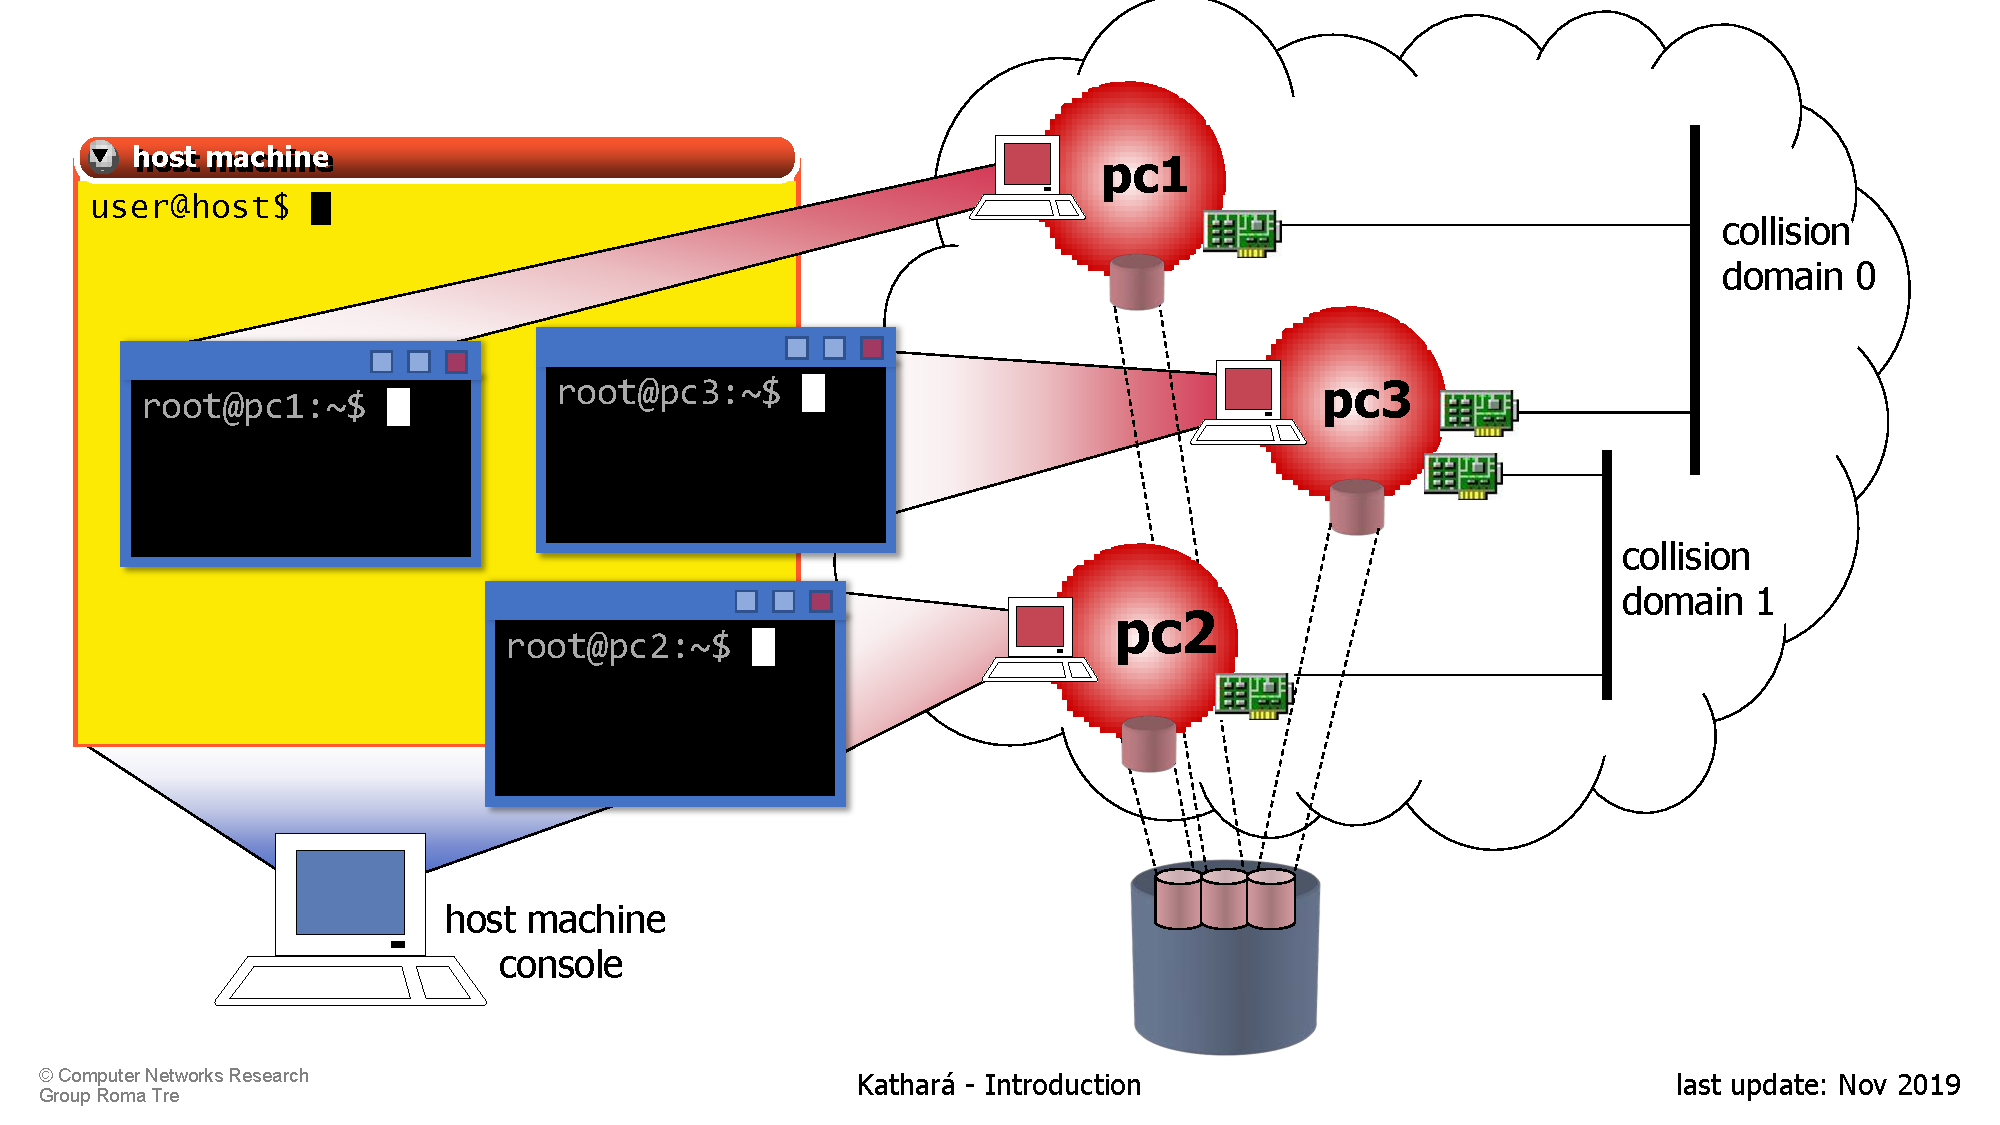
\includegraphics[width=0.8\textwidth,frame]{kathara-topologynodes}
  \caption{Slide taken from `Introduction to Kathará' showing a simplified lab in action}
  \label{fig:kathara-topologynodes}
\end{figure}


As stated in `Introduction to Kathará,' each (emulated) device has:
\begin{itemize}
  \item a console (a terminal window) which gives access to a \texttt{bash} shell inside the container
  \item an (virtually) isolated memory
  \item a (virtually) isolated filesystem, though Kathará provides a way to mount shared files among the nodes of the lab, via a convention of directory hierarchies so no explicit configuration is needed
  \item zero, one, or more network interfaces
\end{itemize}

The slides also explain that each network interface can be connected to a (virtual) collision domain and each virtual collision domain can be connected to several interfaces.
All this is illustrated by figure~\ref{fig:kathara-topologynodes}.

Kathará's interface has two parts: a set of commands that can be issued in the host (the machine where the emulator is being executed) shell, and the a structured way to define labs, which includes a syntax for defining topologies---i.e. which nodes are there, what are their names, how many network interfaces do they have and to which collision domain, aka links, are they connected to---and also a conventionalized way to structure configuration files that are automatically read by the software inside the nodes, like IP configurations or routing parameters.

These interfaces are not exhaustively exposed in this work since that would just mean duplicating the documentation resources, which are easily accessible and very clear.
However, figure~\ref{fig:kathara-topologynodes} serves as a way to illustrate, in contrast with graphical interactive tools, the way topologies are described and allows to take an immediate conclusion: to have only point-to-point links, this means that only each two interfaces that are connected via that each link need a separate collision domain and local-area networks of interconnected $N$ Ethernet-equiped hosts need a switch between them.

What was just said poses a question that will be further explored in the practical case study (section~\ref{sec:katharapracticalcasestudy}): there aren't conventional (layer-2) switching labs in the aforementioned repository, and the routing ones assume that more than one hosts sharing the same IP-prefix simply share collision domains.

% Figure fig:kathara-topologynodes
\begin{figure}
  \centering
  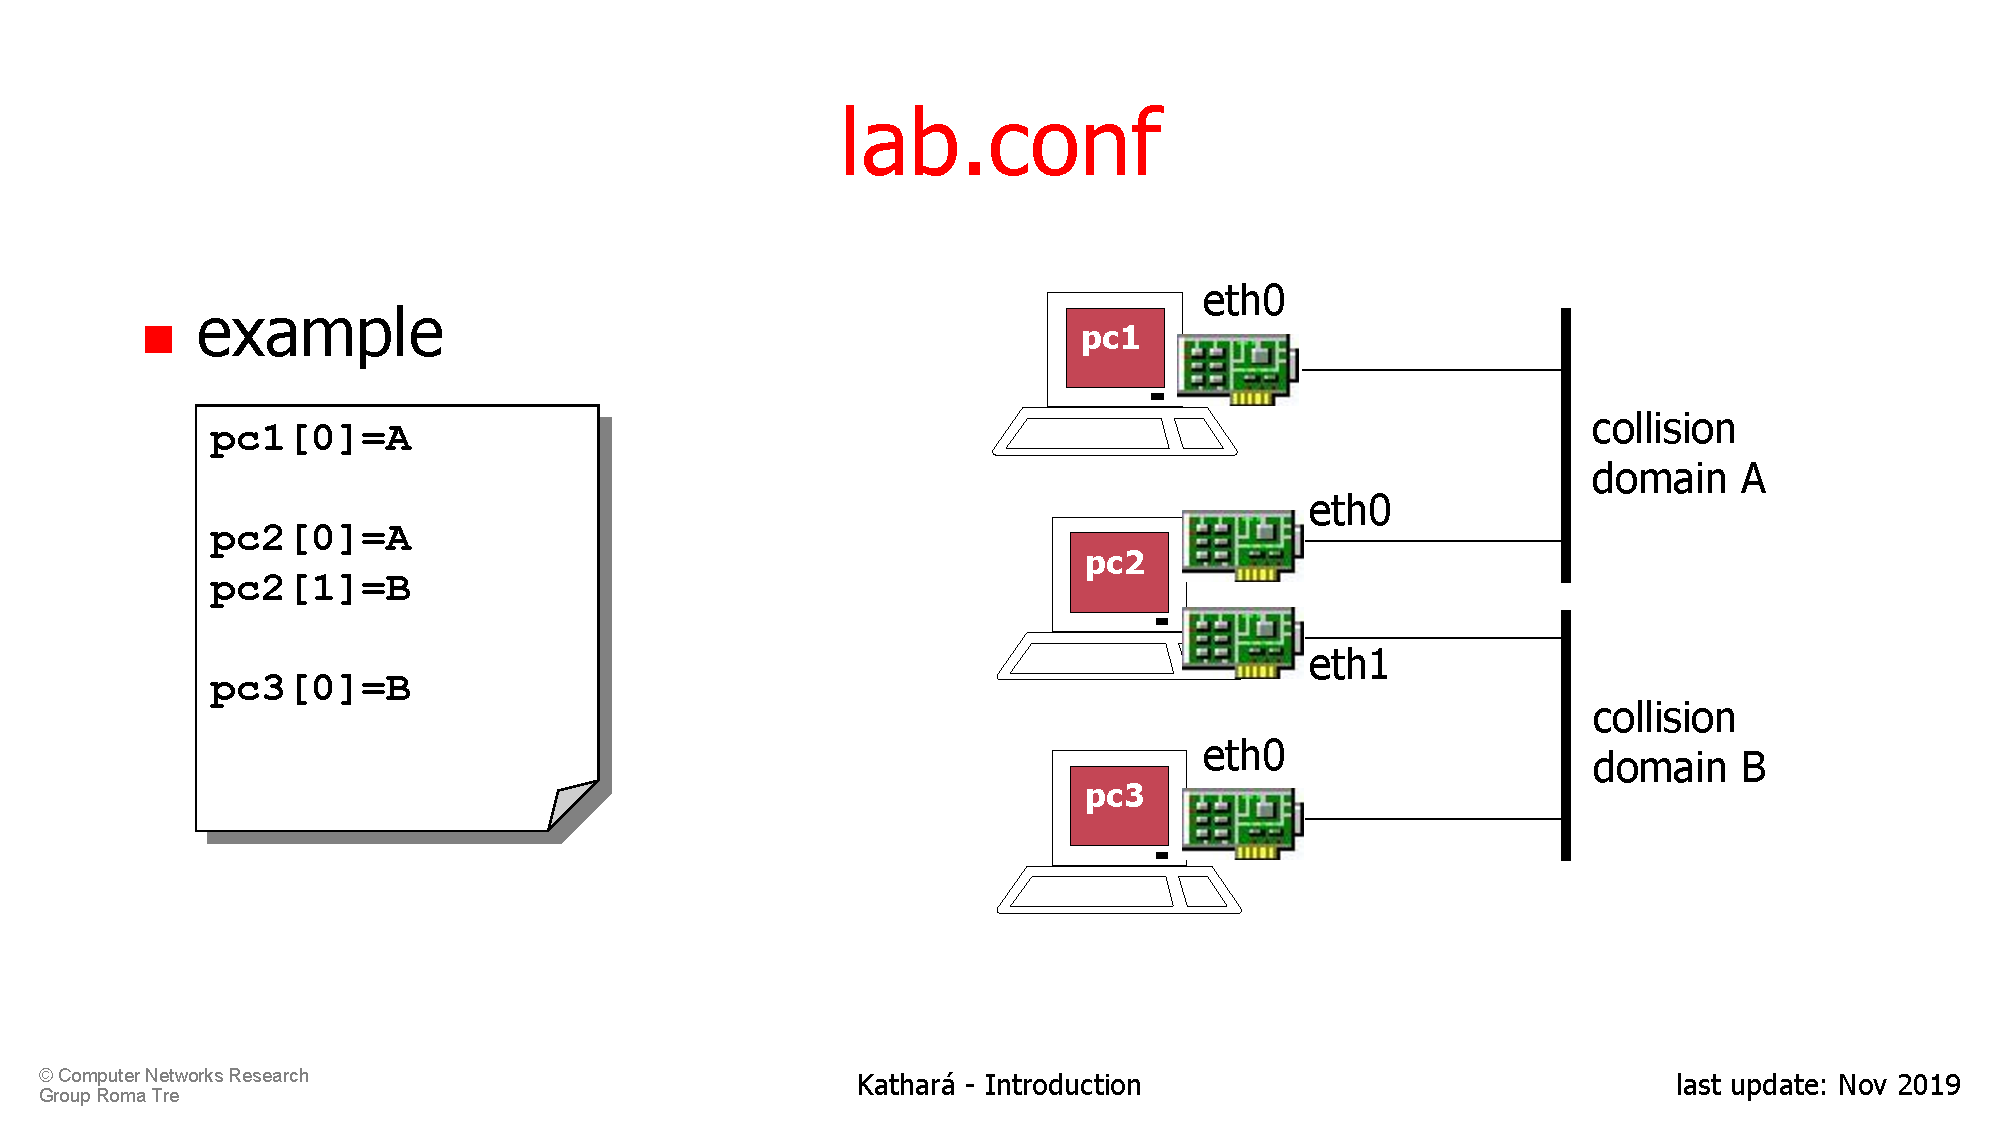
\includegraphics[width=0.8\textwidth,frame]{kathara-labconf}
  \caption{Slide taken from `Introduction to Kathará' showing the mapping between \texttt{lab.conf} and the instantiated topology}
  \label{fig:kathara-labconf}
\end{figure}


% end of section katharafunctionality
